\section{Auswertung}
\label{sec:Auswertung}
Die in \autoref{sec:Auswertung} gezeigten Grafiken und Rechnungen sind mithilfe der Python-Bibliotheken Matplotlib \cite{matplotlib}, Scipy \cite{scipy} und Numpy \cite{numpy}
erstellt worden. Die Fehlerrechnung wird mithilfe der Python-Bibliothek Uncertainties \cite{uncertainties} durchgeführt.

\subsection{Messung der Resonanzfeldstärke der Sweep Spule}
\label{sec:Resonanzfeldstärke}
Für die Messung der Resonanzfeldstärke der Sweep Spule wurde die Apparatur manuell so eingestellt, dass parallel zu der Nord-Süd-Achse des Erdmagnetfeldes steht. Zusätzlich musste die Vertikalkomponente 
des Erdmagnetfeldes kompensiert werden, was durch Einstellen des Stromes in der Vertikalspule erreicht wurde. Der Strom in dieser Spule wurde auf $I_{\text{vertikal}} = \SI{0.244}{\ampere}$ gestellt,  was nach Gleichung (ref) einer magnetischen Feldstärke von $B_{\text{vertikal}} \approx \SI{37.39}{\micro\tesla}$ entspricht.
Die Messwerte für die Messung der Resonanzfeldstärke sind in \autoref{tab:Resonanzfeldstärke} zu sehen. 
\begin{table}[H]
  \centering
  \caption{Frequenz, Stromstärke der Resonanzfeldstärke der Sweep Spule und Spannung der Horizontalen Spule.}
  \label{tab:Resonanzfeldstärke}
  \begin{tabular}{S[table-format=3] | S[table-format=2(2)] | S[table-format=2(2)] | S[table-format=2(2)] | S[table-format=2(2)]}
      \toprule
      {$f  \, \, \left[\mathrm{kHz}\right]$} & {$ I_\text{P1} \, \, \left[ \mathrm{A}\right]$} & {$ I_\text{P1} \, \, \left[ \mathrm{A}\right]$} & {$ U_\text{ho, 1} \, \, \left[ \mathrm{mV}\right]$} & {$ U_\text{ho, 2} \, \, \left[ \mathrm{mV}\right]$}\\
      \midrule
      100 & 0.0599& 0.0724&0& 0 \\ 
      200 &0.071& 0.0947&4.8& 4.8 \\ 
      300 &0.0464& 0.0821&21.7& 21.7 \\ 
      400 &0.0416& 0.0891&31.7& 31.7 \\ 
      500 &0.0258& 0.0853&45.5& 45.5 \\ 
      600 & 0.0275& 0.0986&53.2& 53.2 \\ 
      700 & 0.05& 0.0759&62.4& 73.7 \\ 
      800 &0.0274& 0.0943&69.9& 79.5 \\ 
      900 &0.0236& 0.0743&79.5& 102.6 \\ 
      1000&0.0393& 0.084&82.4& 108.2 \\ 
      \bottomrule
  \end{tabular}
\end{table}
\newpage
\noindent
Die Spannung der horizontalen Spule lässt sich nach 
\begin{equation}
  I_{\text{ho}} = \frac{2 \cdot U_{\text{ho} }}{1000}
\end{equation}
in den Strom der horizontalen Spule umrechnen. Aus den Strömen in der Sweep und horizontalen Spule lassen sich die Magnetfelder der beiden Spulen nach (ref) berechnen.
Dabei sind $N_H = 154$ und $R_H = \SI{0.1579}{m}$ die Windungszahl und der Radius der horizontalen Spule und $N_S = 11$ und $R_S = \SI{0.1639}{m}$ die Windungszahl und der Radius der Sweep Spule.
Die Magnetfelder der beiden Spulen werden addiert und sind in \autoref{fig:Resonanzfeldstärke} gegen die Frequenz aufgetragen. Dabei ist die Feldstärke $B$ die Feldstärke im Resonanzfall bei gegebener Frequenz $f$.
\begin{figure}[H]
  \centering
  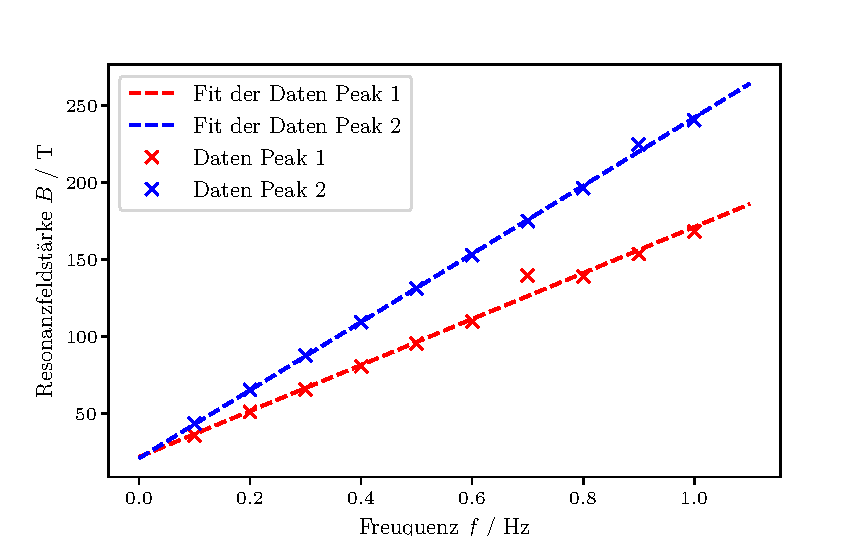
\includegraphics[width=0.8\linewidth]{build/plot1.pdf}
  \caption{Resonanzfeldstärke der Sweep Spule in Abhängigkeit der Frequenz.}
  \label{fig:Resonanzfeldstärke}
\end{figure}
\noindent
Die Daten werden durch eine Funktion der Form 
\begin{equation}
  B(f) = a \cdot f + b
\end{equation}
gefittet, wobei sich die Parameter $a$ und $b$ auf
\begin{align*}
  a_1 &\approx \left(1.4923 \pm  0.0551 \right) \cdot 10^{-10} \frac{\mathrm{T}}{\mathrm{Hz}}\\
  b_1 &\approx \left(2.1934 \pm 0.3421 \right) \cdot 10^{-5} \mathrm{T}
\end{align*}
für den ersten Peak und auf 
\begin{align*}
  a_2 &\approx \left(2.2108 \pm  0.0213 \right) \cdot 10^{-10} \frac{\mathrm{T}}{\mathrm{Hz}}\\
  b_2 &\approx \left(2.1103 \pm 0.1319 \right) \cdot 10^{-5} \mathrm{T}
\end{align*}
für den zweiten Peak ergeben. $b_1$ und $b_2$ entsprechen dabei der horizontalen Erdmagnetfeldstärke, welche nicht durch das Ausrichten der Apparatur kompensiert werden konnte.
\subsection{Messung des Lande-Faktors und des Kernspins}
Aus $a_1$ und $a_2$ lässt sich nach Gleichung (ref) der Lande-Faktor der beiden Isotope bestimmen.
Dieser ergibt sich für die Messwerte des ersten Peaks auf 
\begin{equation}
  g_{F, 1} = \left(0.479 \pm 0.018 \right)
\end{equation} 
und für die Messwerte des zweiten Peaks auf
\begin{equation}
  g_{F, 2} = \left(0.3232 \pm 0.0031 \right) \, .
\end{equation}
Nach Gleichung (ref) berechnen sich die Theoriewerte der Lande Faktoren für ${}^{85}\text{Rb}$ und ${}^{87}\text{Rb}$ auf 
\begin{align*}
  g_{F, 85, \text{theo}} &= 0.\bar{3} \\
  g_{F, 87, \text{theo}} &= 0.5
\end{align*}
Weswegen der erste Peak dem Isotop ${}^{87}\text{Rb}$ und der zweite Peak dem Isotop ${}^{85}\text{Rb}$ zugeordnet werden kann.
Die Kernspins der beiden Isotope können dann durch Umstellen der Gleichung (ref) auf 
\begin{align*}
  I_{87} &= \left(1.532 \pm 0.026\right) \\
  I_{85} &= \left(2.520 \pm 0.006\right)
\end{align*}
bestimmt werden.
\subsection{Messung des Isotopenverhältnisses}
Für die Messung des Isotopenverhältnisses wurde ein Foto des Oszilloskopes gemacht, welches dabei so eingestellt wurde, dass beide Resonanzpeaks der jeweiligen Isotope gut sichtbar sind.
Zu sehen ist das Foto in \autoref{fig:Oszilloskop}.
\begin{figure}[H]
  \centering
  \includegraphics[width=0.6\linewidth]{build/peaks_len.pdf}
  \caption{In Paint bearbeitetes Foto der Resonanzpeaks auf dem Oszilloskop. \cite{ms_paint}}
  \label{fig:Oszilloskop}
\end{figure}
\noindent
Die Längen der Peaks wurden dafür mit Balken verdeutlicht und ein feines Raster wurde über das Bild gelegt. Es können nun die Länge der Balken in Anzahl an Rasterkästchen bestimmt werden, welche sich auf
\begin{align*}
  l_{1} &=  18 \pm 1 \\
  l_{2} &=  34 \pm 1
\end{align*}
ergeben. Dabei wurde ein Ablesefehler von $\pm 1$ angenommen. Aus den Längen der beiden Peaks lässt sich das Verhältnis der beiden Isotope abschätzen, durch
\begin{equation}
  \frac{N_{85}}{N_{87} + N_{85}} \approx \left( 0.654 \pm 0.014 \right) \, .
\end{equation}

\subsection{abschätzung des quadratischen Zeeman Effekts}
\label{sec:Zeeman}
Die Übergangsenergien der aufgespaltenen Zustände in der Quantenzahl $m_F$ lassen sich nach Gleichung (ref) abschätzen. Dabei sind die Lande-Faktoren der Kernspins der beiden Isotope 
\begin{align*}
  g_{I, 85} &= 0.541224 \\
  g_{I, 87} &= 1.8341933333333 \, 
\end{align*}
\cite{nuc_lande}, und die $\Delta$'s der beiden Isotope
\begin{align*}
  \Delta_{85} &= 3035 \, \frac{\mathrm{Mc}}{\mathrm{s}} \\
  \Delta_{87} &= 6837.7 \, \frac{\mathrm{Mc}}{\mathrm{s}} \,
\end{align*}
\cite{benumof}. Die Übergangsenergien der beiden Isotope lassen sich dann bei der jeweiligen maximalen Feldstärke von 
\begin{align*}
  B_{85} &\approx  240 \, \mathrm{\mu T}\\
  B_{87} &\approx  168 \, \mathrm{\mu T}
\end{align*}
auf 
\begin{align*}
  \Delta E_{85} &=  \left( 3.857 \pm 0.008 \right) 10^{-12} \, \text{eV} \\
  \Delta E_{87} &=  \left( 2.688 \pm 0.035 \right) 10^{-12} \, \text{eV}
\end{align*}
abschätzen. 